\documentclass{beamer}

\usepackage[utf8x]{inputenc}
\usepackage{default}
\usetheme{PaloAlto}
\usecolortheme{seahorse}

\title{Sistemas Digitais 2\\ \textbf{Revisão e tópicos sobre circuitos}\\ \textbf{L. Filomeno  Fernandes}}
\date{Brasíla, 02/2011}
\institute{\textbf{Universidade de Brasília - Faculdade do Gama}} 

\begin{document}

%SLIDE INICIAL DE APRESENTAÇÃO
\begin{frame}
  \titlepage
\end{frame}

%SLIDE == CONTEÚDO PROGRAMATICO
\section{Conteúdo Programático}
\begin{frame}
  \frametitle{Conteúdo Programático}
  \begin{itemize}
   \item Fundamentos dos sistemas seqüenciais.\pause
   \item Desenhos de circuitos lógicos seqüenciais. \pause
   \item Análise de circuitos lógicos seqüenciais. \pause
   \item Dispositivos lógicos programáveis.\pause
   \item Linguagem VHDL.
  \end{itemize}

\end{frame}

%SLIDE == BASICO
\section{Básico}
\begin{frame}
  \frametitle{Básico - Portas lógicas}
\begin{center}
  \textbf{\huge{Porta OR}}
  \begin{columns}[c]
   \begin{column}{5cm}
    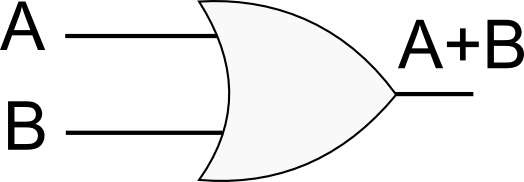
\includegraphics[height = 1in, width = 2in]{or.png}
   \end{column}\pause
   \begin{column}{5cm}
    \begin{tabular}{|c|c|c|}
     \hline
     A & B & A + B \\
     \hline	
     0 & 0 & 0 \\
     0 & 1 & 1 \\
     1 & 0 & 1 \\
     1 & 1 & 1 \\ 
     \hline
    \end{tabular}
   \end{column}

  \end{columns}
\end{center}
\end{frame}

\begin{frame}
  \frametitle{Básico - Portas lógicas}
\begin{center}
   \textbf{\huge{Porta AND}}
   \begin{columns}[c]
   \begin{column}{5cm}
    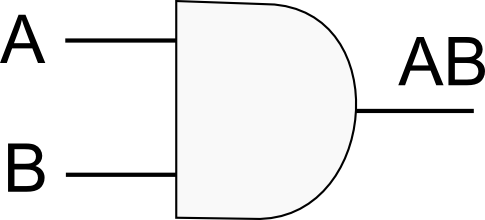
\includegraphics[height = 1in, width = 2in]{and.png}
   \end{column}\pause
   \begin{column}{5cm}
    \begin{tabular}{|c|c|c|}
     \hline
     A & B & AB \\
     \hline	
     0 & 0 & 0 \\
     0 & 1 & 0 \\
     1 & 0 & 0 \\
     1 & 1 & 1 \\ 
     \hline
    \end{tabular}
   \end{column}

  \end{columns}
\end{center}
\end{frame}

\begin{frame}
  \frametitle{Básico - Portas lógicas}
  \begin{center}
    \textbf{\huge{Porta Inversora}}
    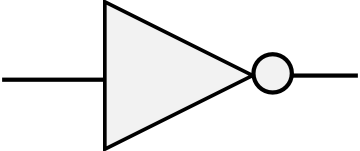
\includegraphics[height = 1in, width = 2in]{inversora.png}
  \end{center}
\end{frame}

\begin{frame}
  \frametitle{Básico - Portas lógicas}
\begin{center}
   \textbf{\huge{Porta NOR}} 
   \begin{columns}[c]
   \begin{column}{5cm}
    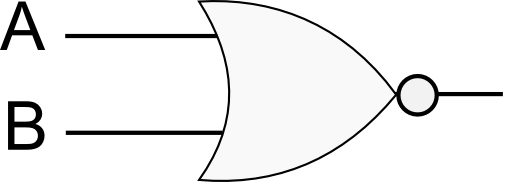
\includegraphics[height = 1in, width = 2in]{nor.png}
   \end{column}\pause
   \begin{column}{5cm}
    \begin{tabular}{|c|c|c|}
     \hline
     A & B & $\overline{A + B}$ \\
     \hline	
     0 & 0 & 1 \\
     0 & 1 & 0 \\
     1 & 0 & 0 \\
     1 & 1 & 0 \\ 
     \hline
    \end{tabular}
   \end{column}

  \end{columns}
\end{center}
\end{frame}

\begin{frame}
  \frametitle{Básico - Portas lógicas}
\begin{center}
   \textbf{\huge{Porta NAND}} 
   \begin{columns}[c]
   \begin{column}{5cm}
    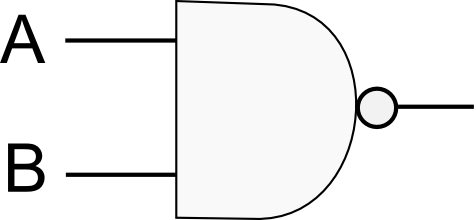
\includegraphics[height = 1in, width = 2in]{nand.png}
   \end{column}\pause
   \begin{column}{5cm}
    \begin{tabular}{|c|c|c|}
     \hline
     A & B & $\overline{AB}$ \\
     \hline	
     0 & 0 & 1 \\
     0 & 1 & 1 \\
     1 & 0 & 1 \\
     1 & 1 & 0 \\ 
     \hline
    \end{tabular}
   \end{column}

  \end{columns}
\end{center}
\end{frame}

\begin{frame}
  \frametitle{Básico - Portas lógicas}
\begin{center}
   \textbf{\huge{Porta XOR}} 
   \begin{columns}[c]
   \begin{column}{5cm}
    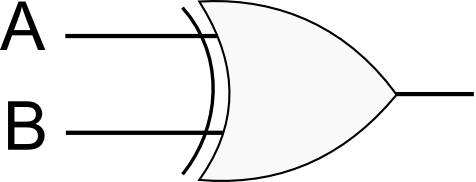
\includegraphics[height = 1in, width = 2in]{xor.png}
   \end{column}\pause
   \begin{column}{5cm}
    \begin{tabular}{|c|c|c|}
     \hline
     A & B & $A \oplus B$ \\
     \hline	
     0 & 0 & 0 \\
     0 & 1 & 1 \\
     1 & 0 & 1 \\
     1 & 1 & 0 \\ 
     \hline
    \end{tabular}
   \end{column}

  \end{columns}
\end{center}
\end{frame}

\begin{frame}
  \frametitle{Básico - Portas lógicas}
\begin{center}
   \textbf{\huge{Porta XNOR}}
   \begin{columns}[c]
   \begin{column}{5cm}
    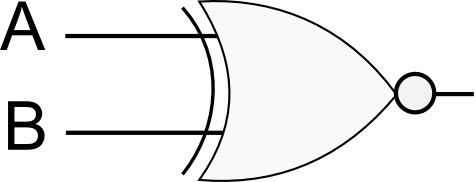
\includegraphics[height = 1in, width = 2in]{xnor.png}
   \end{column}\pause
   \begin{column}{5cm}
    \begin{tabular}{|c|c|c|}
     \hline
     A & B & $\overline{A \oplus B}$ \\
     \hline	
     0 & 0 & 1 \\
     0 & 1 & 0 \\
     1 & 0 & 0 \\
     1 & 1 & 1 \\ 
     \hline
    \end{tabular}
   \end{column}

  \end{columns}
\end{center}
\end{frame}

\begin{frame}
  \frametitle{Básico - Operações booleanas}
\begin{columns}[c]
  \begin{column}{3cm}
   \begin{itemize}
   \item $x.0 = 0 $  \pause
   \item $x.1 = x $  \pause 
   \item $x.x = x $  \pause
   \item $x.\overline{x} = 0 $  \pause
   \item $x + 0 = x $  \pause
   \item $x + 1 = 1 $  \pause 
   \item $x + x = x $  \pause 
   \item $x + \overline{x} = 0 $  \pause 
   \item $x + y = y + x $  \pause 
  \end{itemize}
 \end{column} 
  
  \begin{column}{7cm}
   \begin{itemize}
   \item $x.y = y.x $  \pause
   \item $x + (y + z) = (x + y) + z = x + y + z $  \pause 
   \item $x(yz) = (xy)z = xyz $  \pause
   \item $x(y + z) = xy + xz $  \pause
   \item $(w + x)(y + z) = wy + xy + wz + xz$  \pause
   \item $x + xy = x $  \pause 
   \item $x + \overline{x}y = x + y $  \pause 
   \item $\overline{x} + xy = \overline{x} + y$  \pause 
   \item $\overline{(x + y)} = \overline{x}\overline{y} $  \pause 
   \item $\overline{(xy)} = \overline{x} + \overline{y} $   
  \end{itemize}
  \end{column}
\end{columns}
\end{frame}

%SECAO == CIRCUITOS
\section{Conceitos fundamentais}
\begin{frame}
 \frametitle{Conceitos fundamentais}
 \begin{itemize}
  \item Combinacionais
  \item Sequenciais
 \end{itemize}
\end{frame}

\begin{frame}
 \frametitle{Conceitos fundamentais}
 \begin{itemize}
  \item Circuitos combinacionais: em que a saída depende apenas das condições de entrada e/ou para cada combinação de entradas obtêm-se sempre a mesma saída. 
	Exemplo: seletor de canais de TV.\pause
  \begin{itemize}
   \item Álgebra de Boole. \pause
   \item Tabela verdade. \pause
   \item Mapas de Veitch-Karnaugh.
  \end{itemize}
 \end{itemize}
\end{frame}

\begin{frame}
 \begin{itemize}
  \item Circuitos seqüências: em que a saída depende da combinação de entrada atual bem como das entrada anteriores. \\Exemplo: seletor de canais de TV com botões up/down (+/-).\pause
  \begin{itemize}
   \item Circuitos com memória, dispositivos que permitem o armazenamento de valores (0 ou 1) em suas saídas por um certo tempo mediante o uso de flip-flops.\pause
   \item Autômatos ou máquinas de estado finitas. \pause
   \item Diagramas de estado.
  \end{itemize}

 \end{itemize}
\end{frame}

\begin{frame}
  \frametitle{Conceitos fundamentais}
  \begin{itemize}
   \item \textbf{Circuitos seqüências síncronos:} circuitos em que todos os dispositivos que compõem a memória recebem o mesmo sinal de relógio.\pause
   \item \textbf{Circuitos seqüências assíncronos:} circuitos em que o sinal de relógio não chega ao mesmo tempo a todos os dispositivos que compõem a memória \pause
   \item \textbf{Estado:} o conceito de estado de um circuito define-se como sendo o \textbf{valor de um conjunto de variáveis de estado num tempo específico. O estado contém as 
	 informações das entradas que estejam presentes} até esse tempo específico.  Ou seja, a informação necessária sobre o passado para determinar o comportamento 
	 futuro do circuito.
  \end{itemize}
\end{frame}

\begin{frame}
 \frametitle{Conceitos fundamentais}
 \begin{itemize}
  \item No exemplo dos canais de TV, o número do canal atual é o estado atual.\pause
  \item Dado o estado atual, nós podemos prever o estado seguinte como uma função das entradas.\pause
  \item Em um circuito digital, variáveis de estado são valores binários.\pause
  \item Um circuito com \textbf{\emph{n}} variáveis de estado binário tem ${2^n}$ estados possíveis.
  \item Circuitos seqüências são também chamados máquina de estado  finito (finita).
 \end{itemize}
\end{frame}

\begin{frame}
 \frametitle{Conceitos de período, freqüência e duty cicle}
 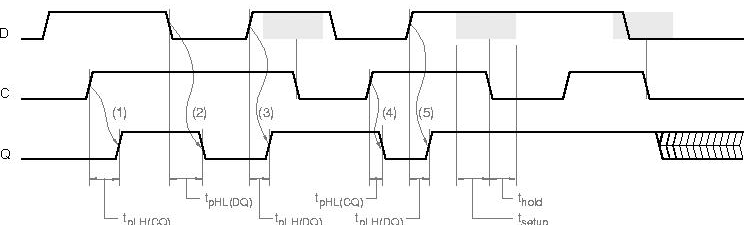
\includegraphics[height = 1.3in, width = 4in]{slide10_filomeno}
 \begin{itemize}
  \item Período do relógio (T)$\xrightarrow{}$ é tempo entre transições sucessivas na mesma direção (subida ou descida).\pause
  \begin{itemize}
   \item Freqüência do relógio$\xrightarrow{}$ é recíproco do período . (f=1/T).\pause
   \item Duty cicle$\xrightarrow{}$ é a percentagem de tempo  do sinal de relógio entre o tempo em alta sobre o tempo em baixa. Duty cicle= tL/tH.
  \end{itemize}
 \end{itemize}
\end{frame}

\begin{frame}
 \frametitle{Tipos de circuitos seqüênciais}
 \begin{itemize}
  \item Dois tipos de circuitos seqüências:\pause
  \begin{itemize}
   \item Circuitos seqüências com realimentação usam portas lógicas e loops (ciclos) de realimentação para obter elementos de memória (latches e flip-flops).\pause
   \item Máquinas de estado síncronas usam latches e flip-flops para criar circuitos que são controlados por um sinal de clock.
  \end{itemize}
 \end{itemize}
\end{frame}

\begin{frame}
 \frametitle{Elementos biestáveis}
 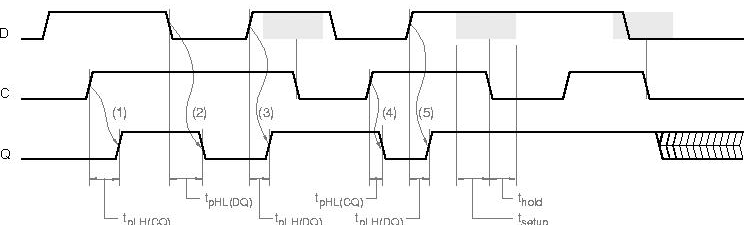
\includegraphics[height = 1.3in, width = 4in]{slide12_filomeno} 
 \begin{itemize}
  \item Atrasos existem para sinais que se propagam das entradas para a saída Q.\pause
  \item Existe uma janela de tempo (tempo de setup e tempo de hold) em torno da borda de descida de C quando a entrada D não deve ser mudada.\pause
  \item A saída do latch é imprevisível, se aqueles tempos não forem.
 \end{itemize}
\end{frame}

\begin{frame}
 \frametitle{Elementos biestáveis}
 \begin{center}
  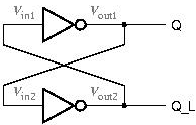
\includegraphics[height = 0.7in, width = 1.3in]{slide13_filomeno} 
 \end{center}
 \begin{itemize}
  \item O circuito seqüencial mais simples consiste de um par de portas inversoras formando um loop com realimentação.\pause
  \item Se Q é ALTO, o inversor de baixo tem uma saída BAIXA, que força o inversor de cima para uma saída ALTA (como foi assumido inicialmente).O circuito é chamado 
	de bi-estável, pois uma análise digital mostra que ele possui dois estados estáveis.
 \end{itemize}
\end{frame}

\begin{frame}
 \frametitle{Elementos biestáveis}
 \begin{center}
  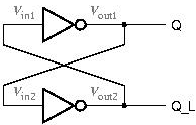
\includegraphics[height = 0.7in, width = 1.3in]{slide13_filomeno} 
 \end{center}
 \begin{itemize}
  \item Se Q é BAIXO, o inversor de baixo tem uma saída ALTA, que força o inversor de cima a produzir uma saída BAIXA (como foi assumido inicialmente. \pause
  \item Nós podemos usar uma variável de estado única (sinal Q) para descrever o estado do circuito. Existem dois estados possíveis, Q=0 e Q=1.
 \end{itemize}
\end{frame}

\begin{frame}
  \frametitle{Elementos biestáveis}
 \begin{center}
  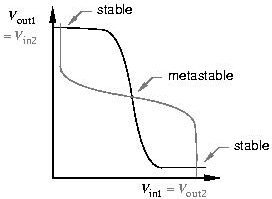
\includegraphics[height = 0.7in, width = 1in]{slide14_filomeno} 
 \end{center}
 \begin{itemize}
  \item O elemento bi-estável é tão simples que ele não tem nenhuma entrada, portanto o seu estado não pode ser controlado.\pause
  \item Quando o circuito é alimentado, ele gera um estado aleatório e permanece nele para sempre.\pause
  \item A análise do bi-estável de uma perspectiva analógica mostra mais aspectos.\pause
  \item O bi-estável está em equilíbrio se as tensões de entrada e saída de ambos inversores são valores constantes consistente com as conexões do loop e as 
	funções de transferência.
 \end{itemize}
\end{frame}

\begin{frame}
  \frametitle{Elementos biestáveis}
 \begin{center}
  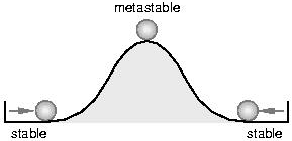
\includegraphics[height = 0.5in, width = 1in]{slide15_filomeno} 
 \end{center}
 \begin{itemize}
  \item O bi-estável está em equilíbrio nos pontos marcados “estável (stable)”.\pause
  \item O terceiro ponto de equilíbrio, chamado “meta-estável (metastable)”, ocorre quando Vout1 e Vout2 não têm nível lógico válido.\pause
  \item Se o circuito opera no ponto metaestável (metastable)”, ele pode permanecer lá  indefinidamente.\pause
  \item O ponto é META-estável, porque ruído aleatório tentará levar o circuito para um ponto estável.\pause
  \item Analogia da bola e colina é usada para ponto meta-estável (metastable)”.
 \end{itemize}
\end{frame}

\begin{frame}
  \frametitle{Elementos biestáveis}
 \begin{center}
  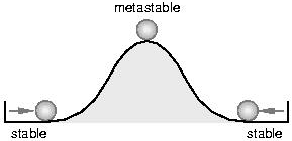
\includegraphics[height = 0.5in, width = 1in]{slide15_filomeno} 
 \end{center}
 \begin{itemize}
  \item O bi-estável está em equilíbrio nos pontos marcados “estável (stable)”.\pause
  \item O terceiro ponto de equilíbrio, chamado “meta-estável (metastable)”, ocorre quando Vout1 e Vout2 não têm nível lógico válido.\pause
  \item Se o circuito opera no ponto metaestável (metastable)”, ele pode permanecer lá  indefinidamente.\pause
  \item O ponto é META-estável, porque ruído aleatório tentará levar o circuito para um ponto estável.\pause
  \item Analogia da bola e colina é usada para ponto meta-estável (metastable)”.
 \end{itemize}
\end{frame}

\section{Flip-flops e Latches}
\begin{frame}
 \frametitle{Flip-flops e Latches}
 \begin{itemize}
  \item Flip-flops e latches  são os blocos básicos utilizados na maioria dos circuitos lógicos seqüências.\pause
  \item Um \textbf{flip-flop} é um dispositivo seqüencial que pega uma amostra da sua entrada e muda a sua saída apenas em instantes de tempo determinado por um 
	sinal de clock.\pause
  \item Um \textbf{latch} é um dispositivo seqüencial que analisa todas as suas entradas continuamente e muda a sua saída em qualquer instante de tempo.
 \end{itemize}
\end{frame}

\begin{frame}
  \frametitle{Latches S-R}
 \begin{center}
  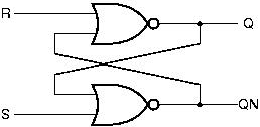
\includegraphics[height = 0.5in, width = 1in]{slide17_filomeno} 
  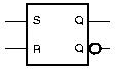
\includegraphics[height = 0.5in, width = 0.8in]{slide17_filomeno2} 
  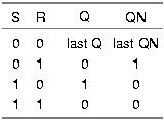
\includegraphics[height = 0.5in, width = 0.8in]{slide17_filomeno3} 
 \end{center}
 \begin{itemize}
  \item Um latch S-R pode ser construído com portas NOR e NAND.\pause
  \item QN é geralmente o complemento de Q.\pause
  \item Se S e R são ambos 0, o circuito comporta como o elemento bi-estável.\pause
  \item Ou S ou R deve ser ativado para forçar o loop (ciclo) de realimentação para um estado desejado.\pause
  \item S set ou coloca a saída Q em 1.\pause
  \item R reset ou coloca a saída que Q em 0.
 \end{itemize}
\end{frame}

\begin{frame}
  \frametitle{Latches S-R}
 \begin{center}
  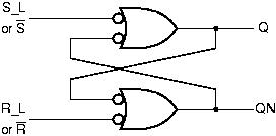
\includegraphics[height = 0.5in, width = 1in]{slide18_filomeno} 
  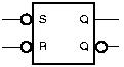
\includegraphics[height = 0.5in, width = 0.8in]{slide18_filomeno2} 
  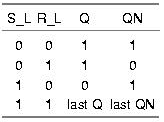
\includegraphics[height = 0.5in, width = 0.8in]{slide18_filomeno3} 
 \end{center}
 \begin{itemize}
  \item Um latch S-R que set e reset as entrada com nível baixo, pode ser construído com portas NAND.\pause
  \item A operação deste latch é similar ao anterior, com duas principais diferenças.\pause
  \item Primeiro, S\_L e R\_L são ativos baixo, assim o latch lembra do seu estado quando S=R=1.\pause
  \item Segundo, quando S\_L e R\_L estão ambos ativos, as duas saídas vão para 1 (not 0).
 \end{itemize}
\end{frame}

\begin{frame}
  \frametitle{Latches S-R}
 \begin{center}
  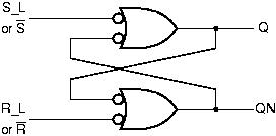
\includegraphics[height = 0.5in, width = 1in]{slide18_filomeno} 
  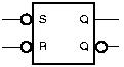
\includegraphics[height = 0.5in, width = 0.8in]{slide18_filomeno2} 
  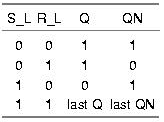
\includegraphics[height = 0.5in, width = 0.8in]{slide18_filomeno3} 
 \end{center}
 \begin{itemize}
  \item Um latch S-R que set e reset as entrada com nível baixo, pode ser construído com portas NAND.\pause
  \item A operação deste latch é similar ao anterior, com duas principais diferenças.\pause
  \item Primeiro, S\_L e R\_L são ativos baixo, assim o latch lembra do seu estado quando S=R=1.\pause
  \item Segundo, quando S\_L e R\_L estão ambos ativos, as duas saídas vão para 1 (not 0).
 \end{itemize}
\end{frame}

\begin{frame}
  \frametitle{Latches S-R}
 \begin{center}
  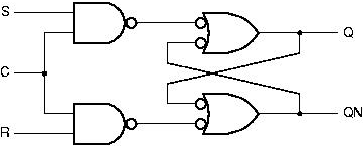
\includegraphics[height = 0.5in, width = 1in]{slide19_filomeno} 
  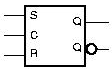
\includegraphics[height = 0.5in, width = 0.8in]{slide19_filomeno2} 
  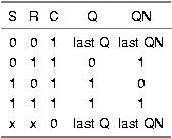
\includegraphics[height = 0.5in, width = 0.8in]{slide19_filomeno3} 
 \end{center}
 \begin{itemize}
  \item Um latch S-R é sensível as suas entradas durante todo o tempo.\pause
  \item Ele pode ser modificado para ser sensível a estas entradas apenas quando uma entrada C for ativada.\pause
  \item O circuito se comporta como um latch S-R quando C=1.\pause
  \item Ele retém o seu estado quando C=0.
 \end{itemize}
\end{frame}

\begin{frame}
  \frametitle{Latches D}
 \begin{itemize}
  \item Latches são necessários para armazenar bits de informação.\pause
  \item Um latch D pode ser usado com este  propósito.\pause
  \item O latch D pode ser construído a partir de um latch S-R.\pause
  \item Este latch elimina a situação problemática em latches S-R, onde S e R podem ser ativados simultaneamente.\pause
  \item Quando C=1, o latch é aberto e a saída Q segue a entrada D. Quando C=0, o latch é fechado.
 \end{itemize}
 \begin{center}
  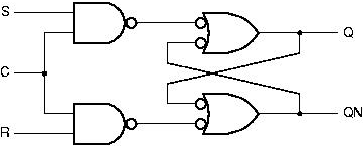
\includegraphics[height = 0.5in, width = 1in]{slide19_filomeno} 
  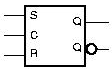
\includegraphics[height = 0.5in, width = 0.8in]{slide19_filomeno2} 
  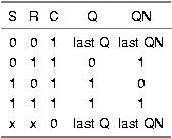
\includegraphics[height = 0.5in, width = 0.8in]{slide19_filomeno3} 
 \end{center}
\end{frame}

\begin{frame}
  \frametitle{Latches D}
 \begin{center}
  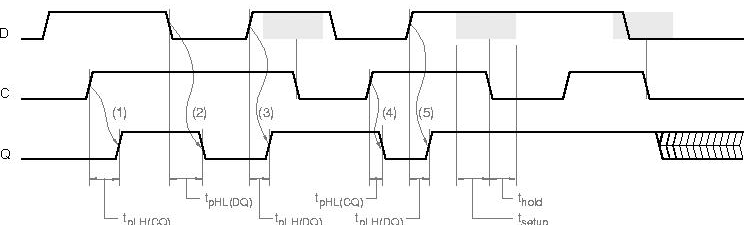
\includegraphics[height = 1.3in, width = 4in]{slide10_filomeno}
 \end{center}
 \begin{itemize}
  \item Atrasos existem para sinais que se propagam das entradas para a saída Q.\pause
  \item Existe uma janela de tempo (tempo de setup e tempo de hold) em  torno da borda de descida de C quando a entrada D não deve ser mudada.\pause
  \item A saída do latch é imprevisível, se aqueles tempos não forem respeitados.
 \end{itemize}
\end{frame}

\begin{frame}
  \frametitle{Flip-Flop D}
 \begin{center}
  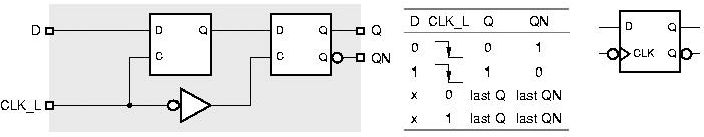
\includegraphics[height = 1in, width = 3.5in]{slide23_filomeno}
 \end{center}
 \begin{itemize}
  \item O triângulo na entrada CLK é um indicador de entrada dinâmica e indica comportamento gatilhado-por-borda.\pause
  \item Um flip-flop D gatilhado-por-borda-negativa simplesmente inverte a entrada clock e a ação ocorre na borda de descida do sinal de clock.
 \end{itemize}
\end{frame}

\begin{frame}
  \frametitle{Flip-Flop D}
 \begin{center}
  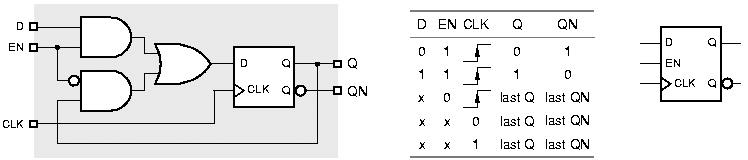
\includegraphics[height = 0.7in, width = 3.5in]{slide24_filomeno}
 \end{center}
 \begin{itemize}
  \item Alguns flip-flops D tem entradas assíncronas que são usadas para forçar o seu estado, independente das entradas CLK e D.\pause
  \item Estas entradas (PR e CLR) se comportam como entradas set e reset do latch S-R.\pause
  \item Elas devem ser usadas para tarefas de inicialização e teste.\pause
  \item Alguns flip-flops D tem a possibilidade de segurar o último estado armazenado. Isto é alcançado adicionando uma entrada enable (habilita).
 \end{itemize}
\end{frame}

\begin{frame}
  \frametitle{Latches S-R}
 \begin{itemize}
  \item Latches S-R são úteis para aplicações de controle, onde podemos ter condições independentes para set/reset um bit de controle.
 \end{itemize}
 \begin{center}
  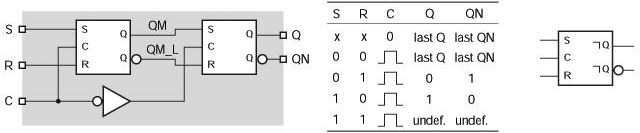
\includegraphics[height = 0.7in, width = 3.5in]{slide25_filomeno}
 \end{center} 
\end{frame}

\begin{frame}
  \frametitle{Flip-flops J-K}
 \begin{itemize}
  \item O problema de ativar S e R simultaneamente é solucionado em um flip-flop J-K mestre-escravo.\pause
  \item As entradas J e K são análogas as entradas S e R.\pause
  \item Entretanto, ativando J aciona a entrada S do mestre somente se Q=0.\pause
  \item Ativando K aciona a entrada mestre R apenas se Q=1.\pause
  \item Assim, se J e K são ativadas simultaneamente, o flip-flop vai para o estado oposto do seu estado atual.
 \end{itemize}
 \begin{center}
  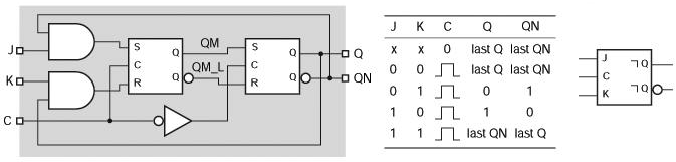
\includegraphics[height = 0.7in, width = 3.5in]{slide26_filomeno}
 \end{center} 
\end{frame}

\begin{frame}
  \frametitle{Flip-flops J-K}
 \begin{itemize}
  \item O problema de ativar S e R simultaneamente é solucionado em um flip-flop J-K mestre-escravo.\pause
  \item As entradas J e K são análogas as entradas S e R.\pause
  \item Entretanto, ativando J aciona a entrada S do mestre somente se Q=0.\pause
  \item Ativando K aciona a entrada mestre R apenas se Q=1.\pause
  \item Assim, se J e K são ativadas simultaneamente, o flip-flop vai para o estado oposto do seu estado atual.
 \end{itemize}
 \begin{center}
  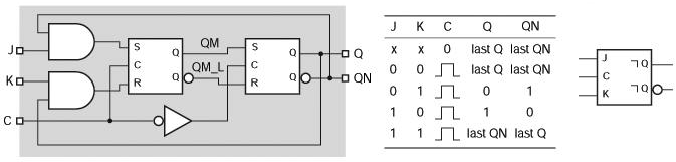
\includegraphics[height = 0.7in, width = 3.5in]{slide26_filomeno}
 \end{center} 
\end{frame}

\begin{frame}
  \frametitle{Flip-flops J-K}
 \begin{center}
  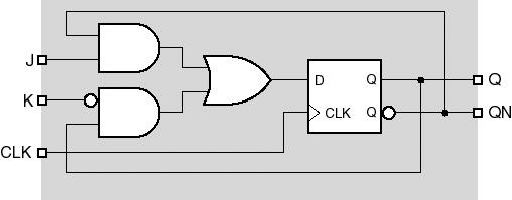
\includegraphics[height = 0.7in, width = 2in]{slide27_filomeno} \\
  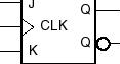
\includegraphics[height = 0.3in, width = 0.5in]{slide27_filomeno2} 
  \@ 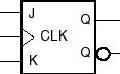
\includegraphics[height = 0.3in, width = 0.5in]{slide27_filomeno3}\\
  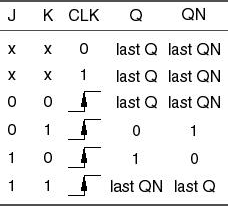
\includegraphics[height = 0.7in, width = 1in]{slide27_filomeno4}
 \end{center} 
\end{frame}

\begin{frame}
  \frametitle{Flip-flops T}
  \begin{center}
  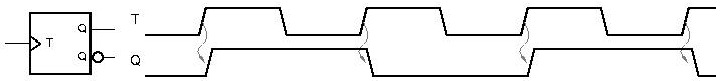
\includegraphics[height = 0.5in, width = 3in]{slide28_filomeno}\\
  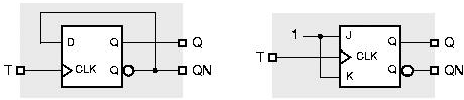
\includegraphics[height = 0.5in, width = 3in]{slide28_filomeno2}
 \end{center} 
 \begin{itemize}
  \item Um flip-flop T muda de estado a cada pulso de clock.\pause
  \item O sinal na saída Q do flip-flop tem metade da freqüência da entrada T.\pause
  \item Flip-flops D e J-K podem ser usados para construir um flip-flop T.
 \end{itemize}
\end{frame}

\begin{frame}
  \frametitle{Flip-flops T}
  \begin{center}
  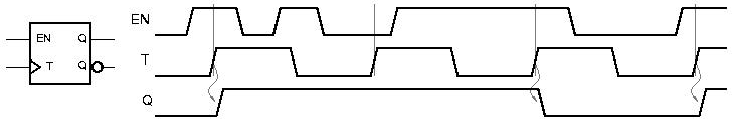
\includegraphics[height = 0.5in, width = 3in]{slide29_filomeno}\\
  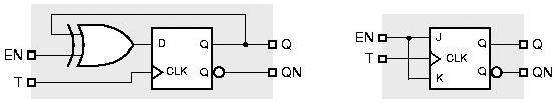
\includegraphics[height = 0.5in, width = 3in]{slide29_filomeno2}
 \end{center} 
 \begin{itemize}
  \item Um flip-flop T pode ter uma entrada enable (habilita).\pause
  \item O flip-flop muda de estado na borda gatilhada do clock, apenas se o sinal enable EM for ativado.\pause
  \item Flip-flops D e J-K podem ser usados para construir um flip-flop T com enable (habilita).
 \end{itemize}
\end{frame}

%SEÇÃO == COLABORADORES
\section{Colaboradores}
\begin{frame}
 \frametitle{Colaboradores}
 \begin{enumerate}
  \item Rodrigo Siqueira de Melo
 \end{enumerate}
\end{frame}

%SLIDE == REFERENCIA BIBLIOGRAFICA
\section{Bibliografia}
\begin{frame}
 \frametitle{Referências bibliográficas}
 \begin{enumerate}
  \item Ewang, E. O., Digital Logic and Microprocessor Design with VHDL, 3o edição, Prentice Hall, 1999.
  \item Tocci, R.J., Widmer, N.S., Moss, G.L. - Sistemas Digitais, Princípios e   Aplicações, 10a Edição, São Paulo: Pearson Prentice Hall, 2007, 804 p., ISBN 9788576050957.
  \item Wakerly, J. F., Digital Designs Principles and Practices, 3o edição, Prentice Hall, 1999.
  \item Mendonça, A. e Zelenovsky, R., Eletrônica Digital: Curso Prático  Exercícios, MZ Editora Ltda., 2004.
 \end{enumerate}
\end{frame}

\end{document}
